\documentclass[11pt,a4paper]{article}
\usepackage[left=0.7in,right=0.7in,bottom=0.7in,top=0.7in]{geometry}

\usepackage[utf8]{inputenc}
\usepackage[english]{babel}
\usepackage{amsmath,bm}
\usepackage{graphicx}
\usepackage{colortbl}
\usepackage{xcolor}
\colorlet{lblue}{blue!50!black}
\usepackage[bookmarks=true,bookmarksnumbered=true,colorlinks=true,linkcolor=lblue,citecolor=lblue,urlcolor=lblue]{hyperref}
\usepackage{subfigure}
\usepackage{booktabs}
\RequirePackage{newtxtext,newtxmath}

\begin{document}
	
	

\section*{AE 6230 -- HW4: Mode Shapes and Responses of 1-D Continuous Systems}

\textbf{Out:} November 15, 2022; \textbf{Due:} November 23, 2022 by 11:59 PM ET in Canvas \\

\subsection*{Guidelines}

\begin{itemize}

    \item Read each question carefully before doing any work;

    \item If you find yourself doing pages of math, pause and consider if there is an easier approach;
	
    \item You can consult any relevant materials;
 
    \item You can discuss solution approaches with others, but your submission must be your own work;

    \item If you have doubts, please ask questions in class, during office hours, and/or Piazza (no questions via email);
	
    \item The solution to each question should concisely and clearly show the steps;

    \item Simplify your results as much as possible;

    \item Box the final answer for each question;        

    \item Submit any code with the solution (but remember to also submit all relevant plots).
	
\end{itemize}

\clearpage 

\subsection*{Problem 1 -- 30 points}

\begin{figure}[htpt!]
	\centering
	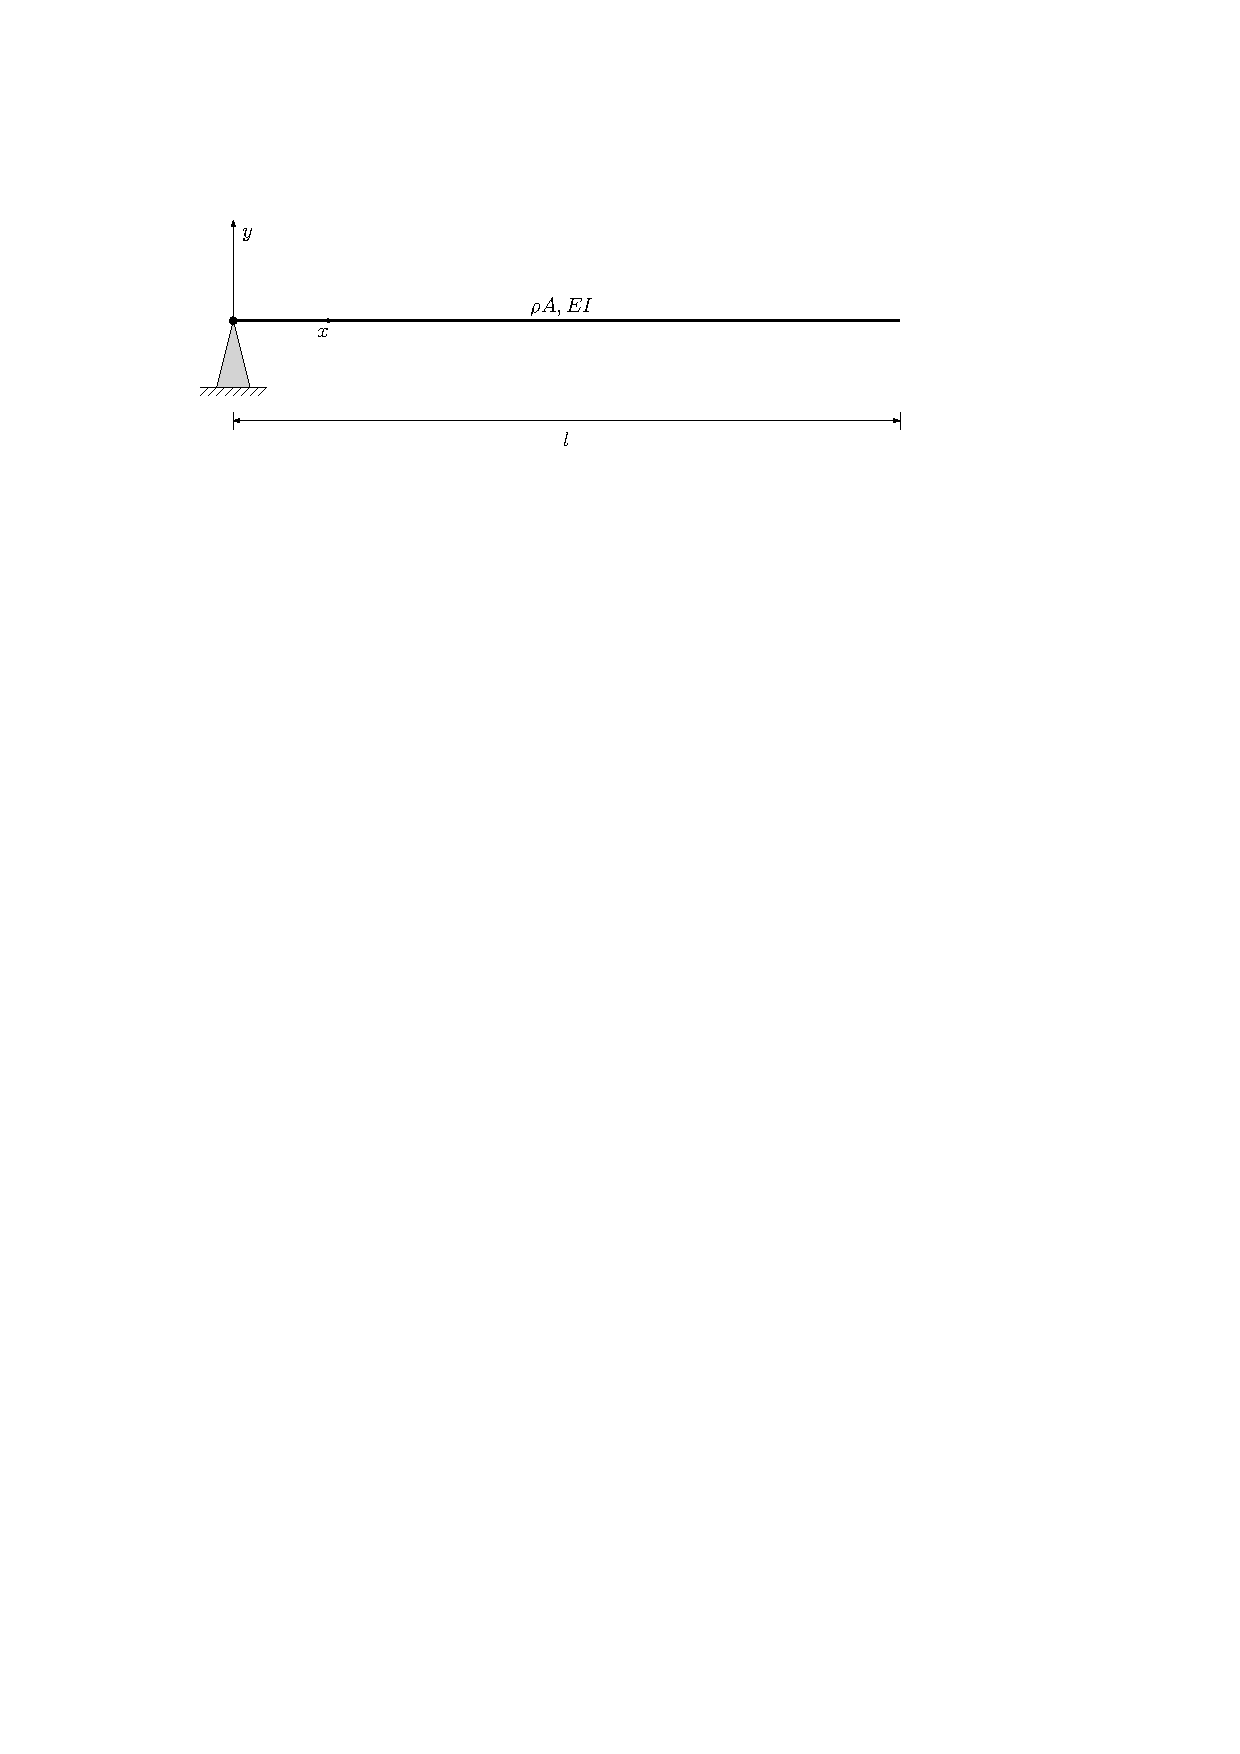
\includegraphics[width=0.8\textwidth]{figures/beam1.pdf}
	\caption{Schematic of a pinned-free uniform beam undergoing out-of-plane bending.}
	\label{f1}
\end{figure}
%
\begin{table}[htpt!]
	\centering
	\caption{Parameter values for Problem 1. \label{t1}}
	\vspace{2mm}
	\begin{tabular}{lrr}
		\toprule
		Parameter & Symbol & Value \\
		\midrule 
		Length & $l$ & 1 m \\
        Bending stiffness & $EI$ & 5 Nm$^2$\\
        Mass per unit length & $\rho A$ & 0.5 kg/m\\
		\bottomrule
	\end{tabular}
\end{table}
%
Figure~\ref{f1} shows a simplified model for the anti-symmetric out-of-plane bending vibrations of an aircraft. Using the anti-symmetry condition, the model considers one half wing represented as a pinned-free uniform beam. Considering the parameters in Table~\ref{t1}, answer the following questions:
%
\begin{enumerate}
    \item Verify that the characteristic equation is given by
    %
    \begin{equation} \label{p1-e1}
    	\tanh \alpha l - \tan \alpha l = 0
    \end{equation}
    %
    \item Evaluate the first four eigenvalues $\alpha_i$;
    \item Evaluate the natural frequencies $\omega_i$;
    \item Determine the analytical expressions of the eigenfunctions $X_i(x)$; 
    \item Plot the mode shapes $\phi_i(x)$ obtained by normalizing the eigenfunctions to have unit maximum displacement;
    \item Verify (mathematically) that there is one rigid-body eigenfunction.
\end{enumerate} 

\clearpage 

\subsection*{Problem 2 -- 15 points}

\begin{figure}[htpt!]
	\centering
	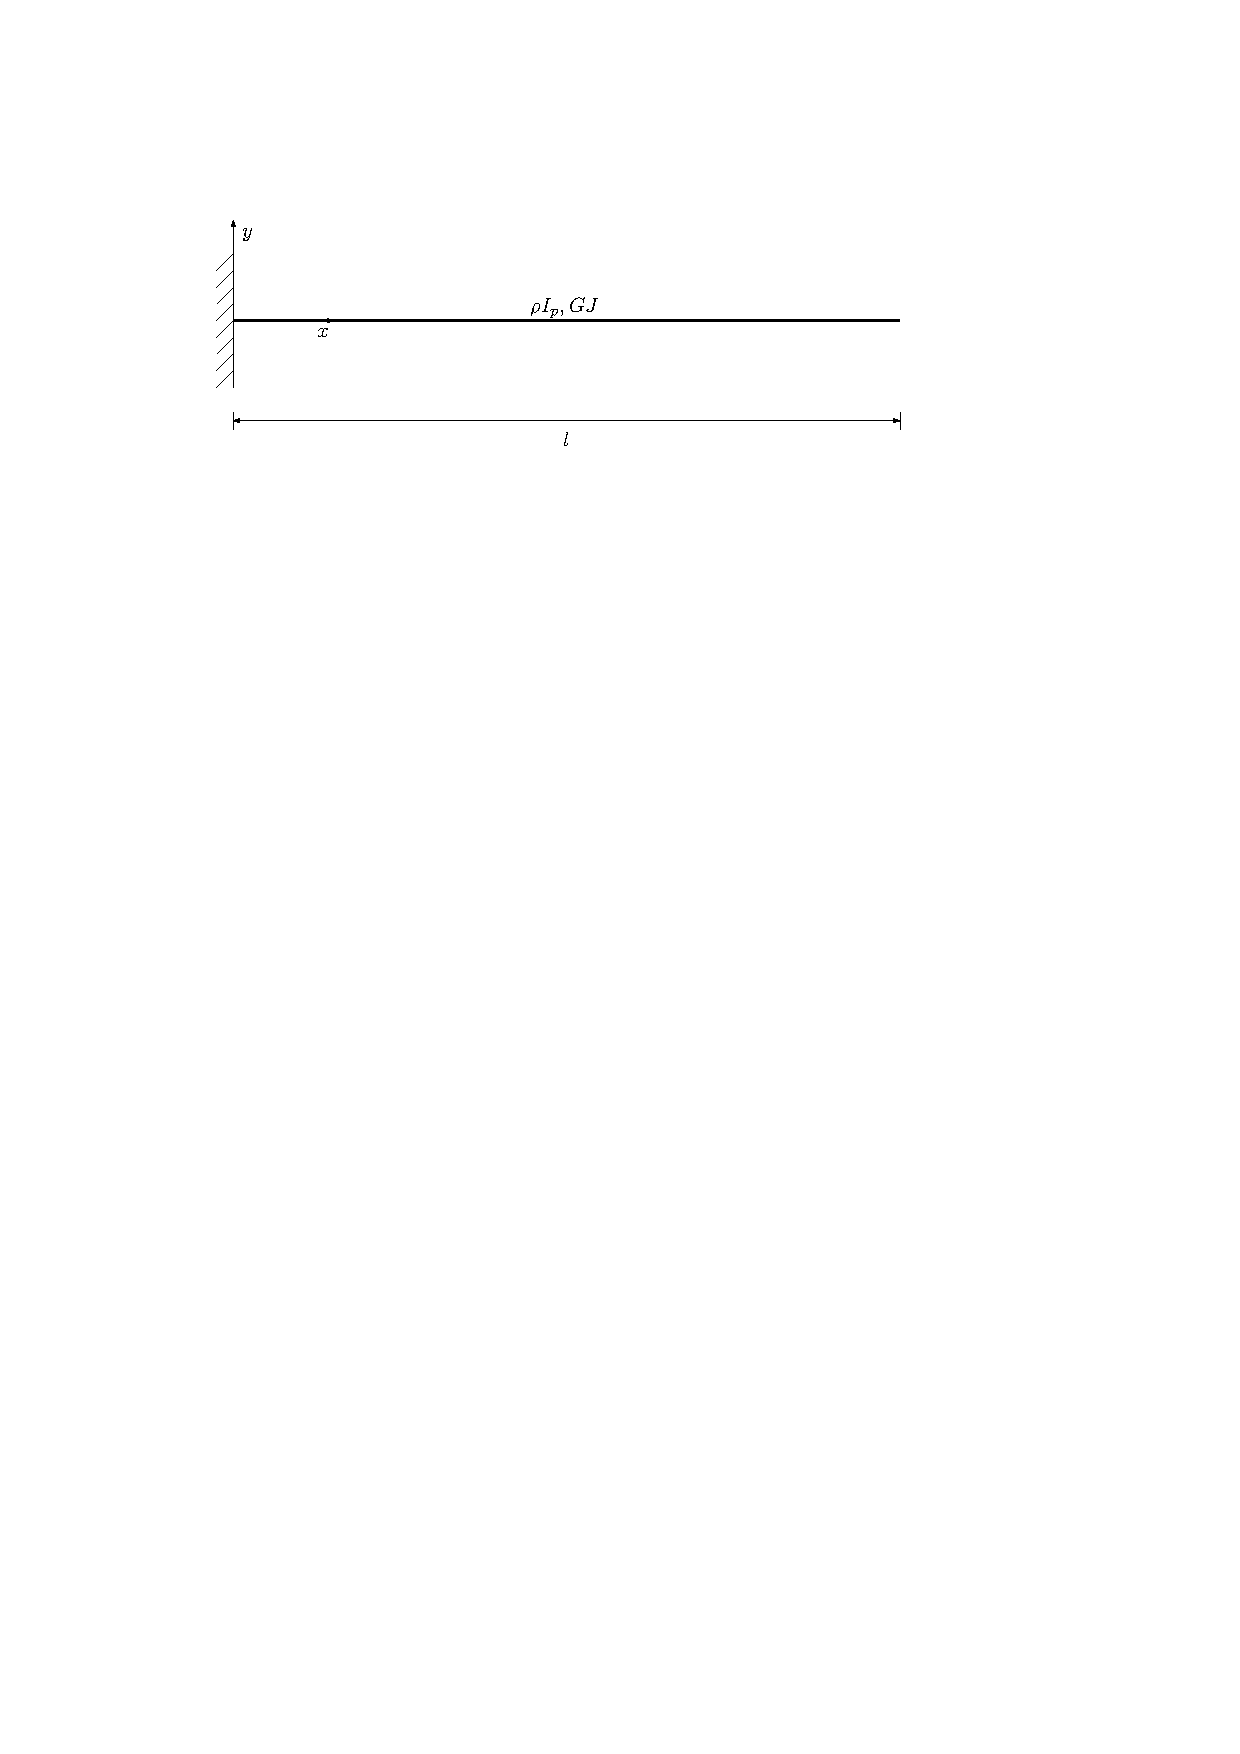
\includegraphics[width=0.8\textwidth]{figures/beam2.pdf}
	\caption{Schematic of a clamped-free uniform beam undergoing torsion.}
	\label{f2}
\end{figure}
%
Figure~\ref{f2} shows a clamped-free uniform beam undergoing torsion. The beam is subject to the initial conditions
%
\begin{equation} \label{p2-e1}
	\theta(x,0) = \theta_0(x) = \frac{\bar{\theta} x}{l} \hspace{10mm} 
	\dot{\theta}(x,0) = \dot{\theta}_0(x) = 0
\end{equation}
%
where $\bar{\theta}$ is the tip twist angle at the initial time. Answer the following questions:
%
\begin{enumerate}
	\item Determine the analytical expressions of the modal initial conditions $\eta_{0_i}, \dot{\eta}_{0_i}$;
	\item Write the undamped free response in the form
	%
	\begin{equation} \label{p2-e2}
		\theta(x,t) = \sum_{i=1}^{\infty} \phi_i(x) \eta_i(t)
	\end{equation}
	%
	showing the appropriate expressions of the mode shapes, natural frequencies, and modal coordinates;
	\item Verify that the response from Question 2 satisfies the initial conditions.
\end{enumerate}

\clearpage 

\subsection*{Problem 3 -- 30 points}

\begin{table}[htpt!]
	\centering
	\caption{Parameter values for Problem 3. \label{t2}}
	\vspace{2mm}
	\begin{tabular}{lrr}
		\toprule
		Parameter & Symbol & Value \\
		\midrule 
		Length & $l$ & 1.0 m \\
		Torsional stiffness & $GJ$ & 5.0 Nm$^2$\\
		Moment of inertia per unit length & $\rho I_p$ & 0.005 kg$\cdot$m\\
		Modal viscous damping factor & $\zeta_i$ & 0.02 \\
		Excitation amplitude & $r_0$ & 1 N \\
		Excitation frequency & $\omega_0$ & 125 rad/s\\
		\bottomrule
	\end{tabular}
\end{table}
%
Consider the beam of Problem 2 but now subject to the distributed moment
%
\begin{equation} \label{p3-e1}
	r(x,t) = r_0 \sin \omega_0 t
\end{equation}
% 
Considering the parameters in Table~\ref{t2}, answer the following question:
%
\begin{enumerate}
	\item Determine the analytical expressions of the modal forces $N_i(t)$;
	\item Write the damped steady-state response in the form
	%
	\begin{equation} \label{p3-e2}
		\theta(x,t) = \sum_{i=1}^{\infty} \phi_i(x) \eta_i(t)
	\end{equation}
	%
	showing the appropriate expressions of the modal coordinates;
	\item Tabulate the quantities needed to evaluate Eq.~\eqref{p3-e2} considering the first four modes\footnote{MATLAB prinouts are acceptable.};
	\item Plot the tip twist angle for $0 \le t \le 0.2$ s considering an increasing number of modes $N = 1, 2, 3, 4$;
	\item Explain the trend in the results for increasing $N$;
	\item How should the distributed moment $r(x,t)$ be shaped to avoid exciting the first torsional vibration mode?
\end{enumerate}

\clearpage 

\subsection*{Problem 4 -- 25 points}

\begin{figure}[htpt!]
	\centering
	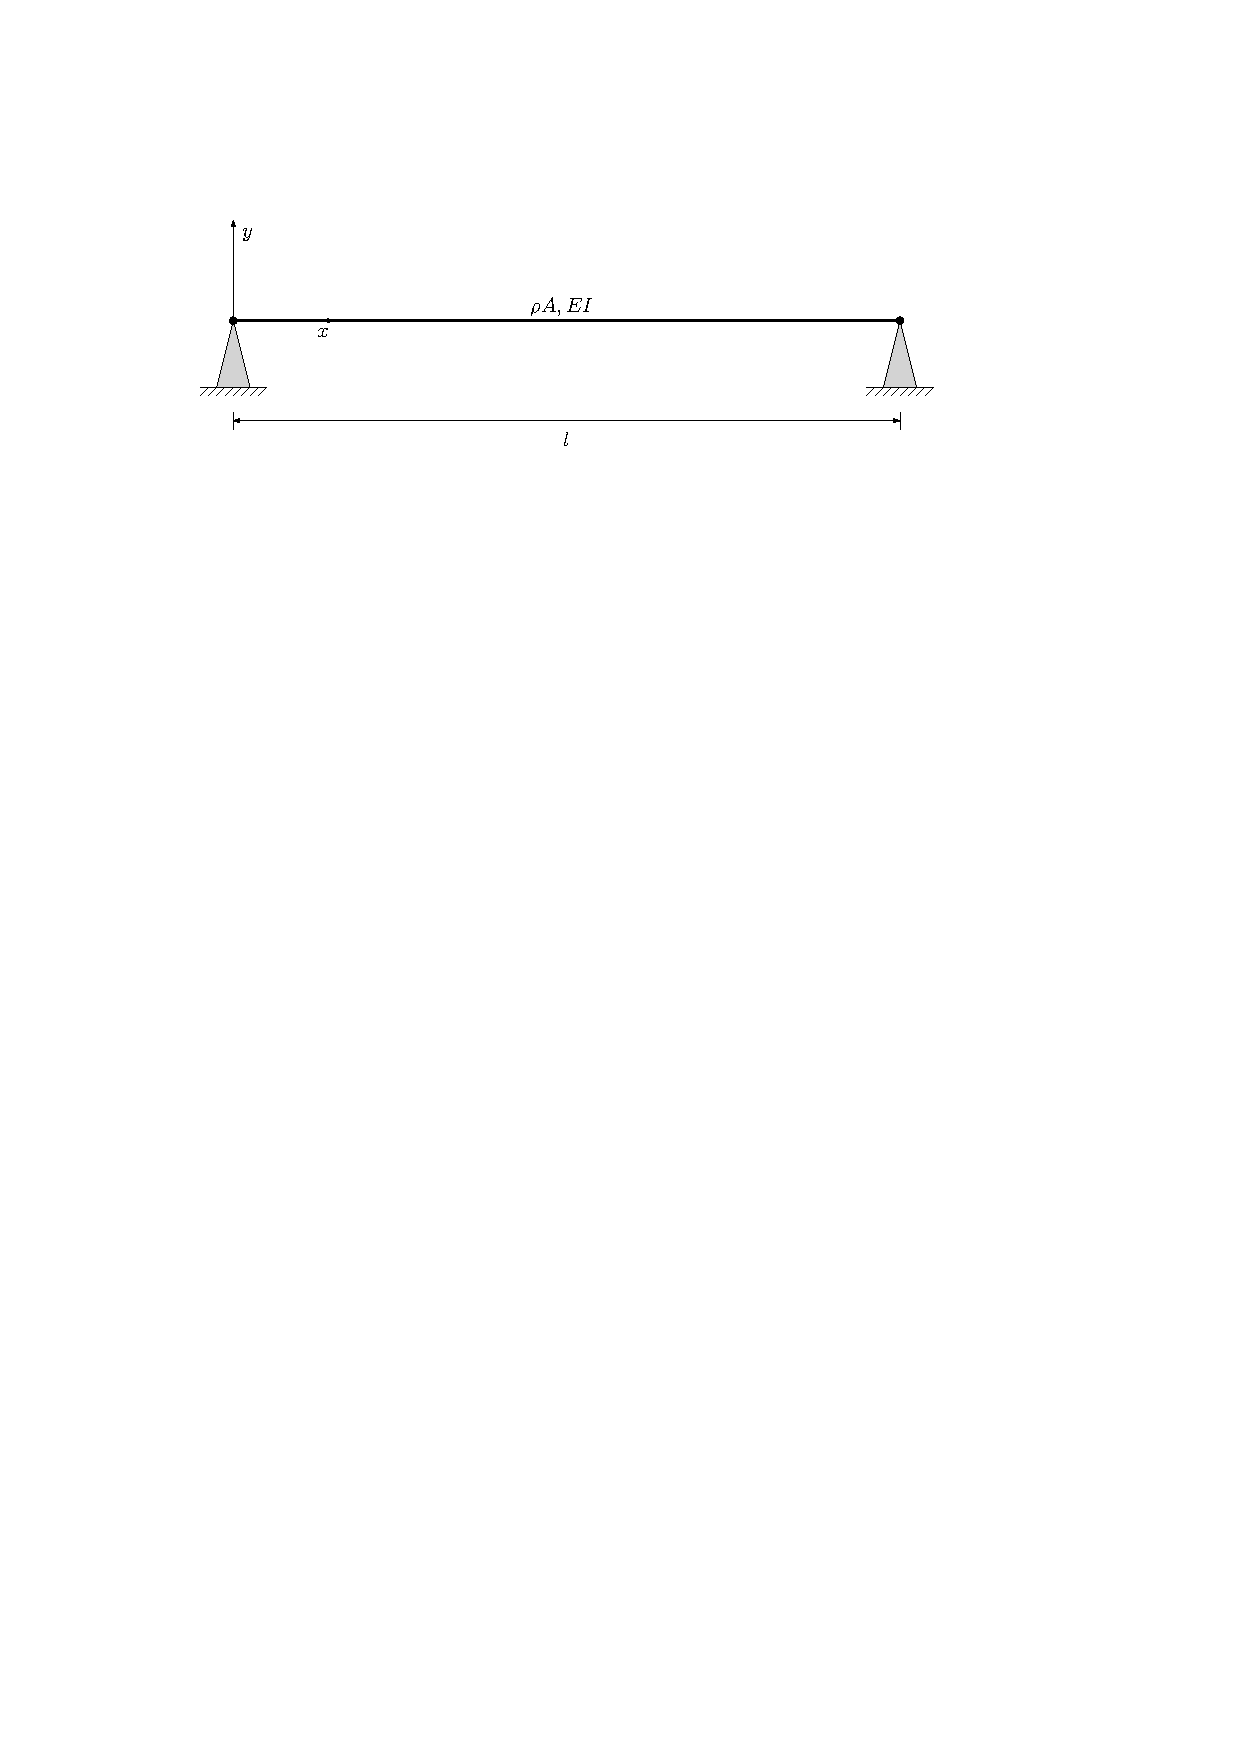
\includegraphics[width=0.8\textwidth]{figures/beam3.pdf}
	\caption{Schematic of a pinned-pinned uniform beam undergoing out-of-plane bending.}
	\label{f3}
\end{figure}
%
\begin{table}[htpt!]
	\centering
	\caption{Parameter values for Problem 4. \label{t3}}
	\vspace{2mm}
	\begin{tabular}{lrr}
		\toprule
		Parameter & Symbol & Value \\
		\midrule 
		Length & $l$ & 1 m \\
		Bending stiffness & $EI$ & 50 Nm$^2$\\
		Mass per unit length & $\rho A$ & 0.25 kg/m\\
		Excitation amplitude & $F_0$ & 1 N\\
		Excitation application point & $x_0$ & $l/2$ \\
		\bottomrule
	\end{tabular}
\end{table}
%
Figure~\ref{f3} shows a pinned-pinned uniform beam in bending. The beam is at rest when it experiences the excitation
%
\begin{equation} \label{p4-e1}
	F(t) = F_0 \, \delta(t) \hspace{5mm} \mathrm{at} \hspace{5mm} x = x_0
\end{equation}
%
where $F_0$ is the amplitude, $x_0$ the application point, and $\delta(t)$ the unit impulse function. The eigenvalues and mode shapes (normalized to have unit maximum displacement) are the same as for a uniform string
%
\begin{equation} \label{p4-e2}
	\alpha_i = \frac{i\pi}{l} \hspace{10mm} 
	\phi_i(x) = \sin\left(\frac{i\pi x}{l}\right)
\end{equation}
%
Considering the parameters in Table~\ref{t3}, answer the following questions:
%
\begin{enumerate}
	\item Determine the analytical expressions of the modal forces $N_i(t)$;
	\item Write the undamped forced response in the form
	%
	\begin{equation} \label{p4-e3}
		v(x,t) = \sum_{i=1}^{\infty} \phi_i(x) \eta_i(t)
	\end{equation}
	%
	showing the appropriate expressions of the natural frequencies and modal coordinates;
	\item Tabulate the quantities needed to evaluate Eq.~\eqref{p4-e2} considering the first eight modes\footnote{MATLAB prinouts are acceptable.};
	\item Plot the midpoint displacement for $0 \le t \le 0.1$ s considering an increasing number of modes $N = 1, \dots, 8$;
	\item Explain the trend in the results for increasing $N$. 
\end{enumerate}

\end{document}

